% tugas_data_analitik_fd001.tex
% Laporan Tugas Data Analitik — C-MAPSS FD001 (Group Submission Version)
% Departemen Teknik Mesin FTUI — 2026

\documentclass[11pt,a4paper]{article}

\usepackage[T1]{fontenc}
\usepackage[utf8]{inputenc}
\usepackage[a4paper, margin=2.5cm]{geometry}
\usepackage{setspace}
\usepackage{parskip}
\usepackage{titlesec}
\usepackage{fancyhdr}
\usepackage{booktabs}
\usepackage{tabularx}
\usepackage{multirow}
\usepackage{graphicx}
\usepackage{caption}
\usepackage{subcaption}
\usepackage{xcolor}
\usepackage{amsmath}
\usepackage{amssymb}
\usepackage{hyperref}
\usepackage{enumitem}
\usepackage{float}
\usepackage{tocloft}
\usepackage{url}

\definecolor{uiblue}{RGB}{0,56,147}
\definecolor{mygray}{RGB}{100,100,100}

\titleformat{\section}
  {\large\bfseries\color{uiblue}}
  {\thesection}{0.6em}{}[\vspace{2pt}\hrule\vspace{4pt}]
\titleformat{\subsection}
  {\normalsize\bfseries\color{uiblue}}{\thesubsection}{0.6em}{}
\titleformat{\subsubsection}
  {\small\bfseries}{\thesubsubsection}{0.6em}{}

\pagestyle{fancy}
\fancyhf{}
\fancyhead[L]{\small\color{mygray}
  Tugas Data Analitik -- Prediksi RUL Mesin Turbofan C-MAPSS FD001}
\fancyhead[R]{\small\color{mygray} Data Analitik 2026}
\fancyfoot[C]{\small\color{mygray}\thepage}
\renewcommand{\headrulewidth}{0.4pt}
\renewcommand{\footrulewidth}{0.0pt}

\onehalfspacing
\captionsetup{font=small, labelfont=bf}
\hypersetup{colorlinks=true, linkcolor=uiblue,
            urlcolor=uiblue, citecolor=uiblue}

% ══════════════════════════════════════════════════════════════════════════════
\begin{document}

% ── Cover ─────────────────────────────────────────────────────────────────────
\begin{titlepage}
  \centering
  \vspace*{1.0cm}
  
\includegraphics[width=2.2cm]{images/logo_ui.png}
  \vspace{0.6cm}

  {\large\bfseries UNIVERSITAS INDONESIA\par}
  \vspace{0.2cm}
  {\normalsize Fakultas Teknik -- Departemen Teknik Mesin\par}

  \vspace{0.5cm}
  \hrule height 1.2pt
  \vspace{0.4cm}
  {\LARGE\bfseries\color{uiblue}
    PREDIKSI \textit{REMAINING USEFUL LIFE}\\[0.3em]
    MESIN TURBOFAN MENGGUNAKAN\\[0.3em]
    \textit{ARTIFICIAL NEURAL NETWORK}\\[0.3em]
    PADA DATASET C-MAPSS FD001\par}
  \vspace{0.4cm}
  \hrule height 1.2pt

  \vspace{1.0cm}
  {\normalsize\color{mygray} Mata Kuliah:\par}
  {\large\bfseries Data Analitik\par}
  \vspace{0.6cm}
  {\normalsize\color{mygray} Dosen Pengampu:\par}
  {\normalsize Dr.\ Eng.\ Sholahudin, S.T., M.Sc.\par}

  \vspace{0.8cm}
  {\normalsize\color{mygray} Disusun Oleh:\par}
  \vspace{0.4cm}
  \begin{tabular}{ll}
    2506565466 & Luqman Alifio Arhab \\[4pt]
    2506565414 & Azfa Rhazasta Abiandra \\[4pt]
    2506565401 & Adamsyah Haryo Saksono \\[4pt]
    2506565433 & Epsiarto Rizqi Nurwijayadi \\[4pt]
  \end{tabular}

  \vspace{0.2cm}
  \vfill
  {\normalsize\bfseries
    DEPARTEMEN TEKNIK MESIN\\
    FAKULTAS TEKNIK\\
    UNIVERSITAS INDONESIA\\[0.4em]
    2026\par}
\end{titlepage}

\thispagestyle{empty}
\newpage
\setcounter{page}{1}
\tableofcontents
\newpage

% ══════════════════════════════════════════════════════════════════════════════
\section{Pendahuluan}

\subsection{Latar Belakang}

Prediksi \textit{Remaining Useful Life} (RUL) merupakan komponen kunci
dalam sistem \textit{Prognostics and Health Management} (PHM). Dengan
mengetahui sisa umur pakai komponen sebelum kegagalan, jadwal perawatan
dapat dioptimalkan sehingga mengurangi biaya \textit{downtime} tak
terencana dan risiko kegagalan mendadak.

\begin{figure}[H]
  \centering
  
\includegraphics[width=0.58\textwidth]{images/01_phm_ecosystem_stack.png}
  \caption{Hierarki PHM --- laporan ini berfokus pada lapisan
    \textit{Prognostics} (prediksi RUL)}
  \label{fig:phm}
\end{figure}

Laporan ini menggunakan sub-dataset \textbf{FD001} dari C-MAPSS NASA:
satu kondisi operasi (\textit{sea level}), satu mode kerusakan (HPC
degradation), 100 mesin \textit{train}, 100 mesin \textit{test}.

\subsection{Tujuan}

\begin{enumerate}[noitemsep]
  \item Membersihkan data dengan analisis korelasi sensor terhadap output (RUL)
  \item Menormalisasi data dengan metode \textit{z-score} berbasis siklus sehat
  \item Memilih fitur menggunakan korelasi Pearson dan PCA
  \item Membangun dan membandingkan model MLP (PCA input vs sensor input)
  \item Menganalisis kepentingan fitur dengan algoritma Garson
\end{enumerate}

\subsection{Alur Pipeline}

\begin{figure}[H]
  \centering\small
  \begin{tabular}{ccccc}
    \fbox{Raw .txt NASA} & $\rightarrow$ &
    \fbox{HDF5} & $\rightarrow$ &
    \fbox{Cleaning} \\[6pt]
    & & & & $\downarrow$ \\[2pt]
    \fbox{Garson} & $\leftarrow$ &
    \fbox{ANN} & $\leftarrow$ &
    \fbox{Normalisasi + PCA}
  \end{tabular}
  \caption{Alur pipeline analitik}
  \label{fig:pipeline}
\end{figure}

% ══════════════════════════════════════════════════════════════════════════════
\section{Dataset C-MAPSS FD001}

\subsection{Deskripsi}

Dataset C-MAPSS dipublikasikan oleh NASA \cite{saxena2008}:
\begin{center}
  \small\url{https://www.nasa.gov/intelligent-systems-division/discovery-and-systems-health/pcoe/pcoe-data-set-repository/}
\end{center}

\begin{figure}[H]
  \centering
  
\includegraphics[width=0.88\textwidth]{images/03_cmapss_engine_schematic.png}
  \caption{Skema mesin turbofan C-MAPSS --- 21 sensor mengukur kondisi
    di sepanjang aliran udara; HPC adalah komponen yang terdegradasi
    pada FD001}
  \label{fig:engine}
\end{figure}

FD001 terdiri dari 20.631 baris data \textit{train} (100 mesin,
siklus penuh hingga kegagalan) dan 13.096 baris \textit{test}
(100 mesin, dipotong sebelum kegagalan). Setiap baris memiliki
26 kolom: \texttt{unit\_number}, \texttt{time\_cycles}, 3
\textit{op\_settings}, dan 21 sensor.

\subsection{Konsep RUL dan Struktur File}

\begin{figure}[H]
  \centering
  
\includegraphics[width=0.85\textwidth]{images/10_train_test_rul_relationship.png}
  \caption{Hubungan antara file train, test, dan RUL ---
    data \textit{test} dipotong di $t^*$;
    \texttt{RUL\_FD001.txt} berisi kunci jawaban}
  \label{fig:rul_rel}
\end{figure}

\subsection{Motivasi: Mengapa RUL Sulit Diprediksi}

\begin{figure}[H]
  \centering
  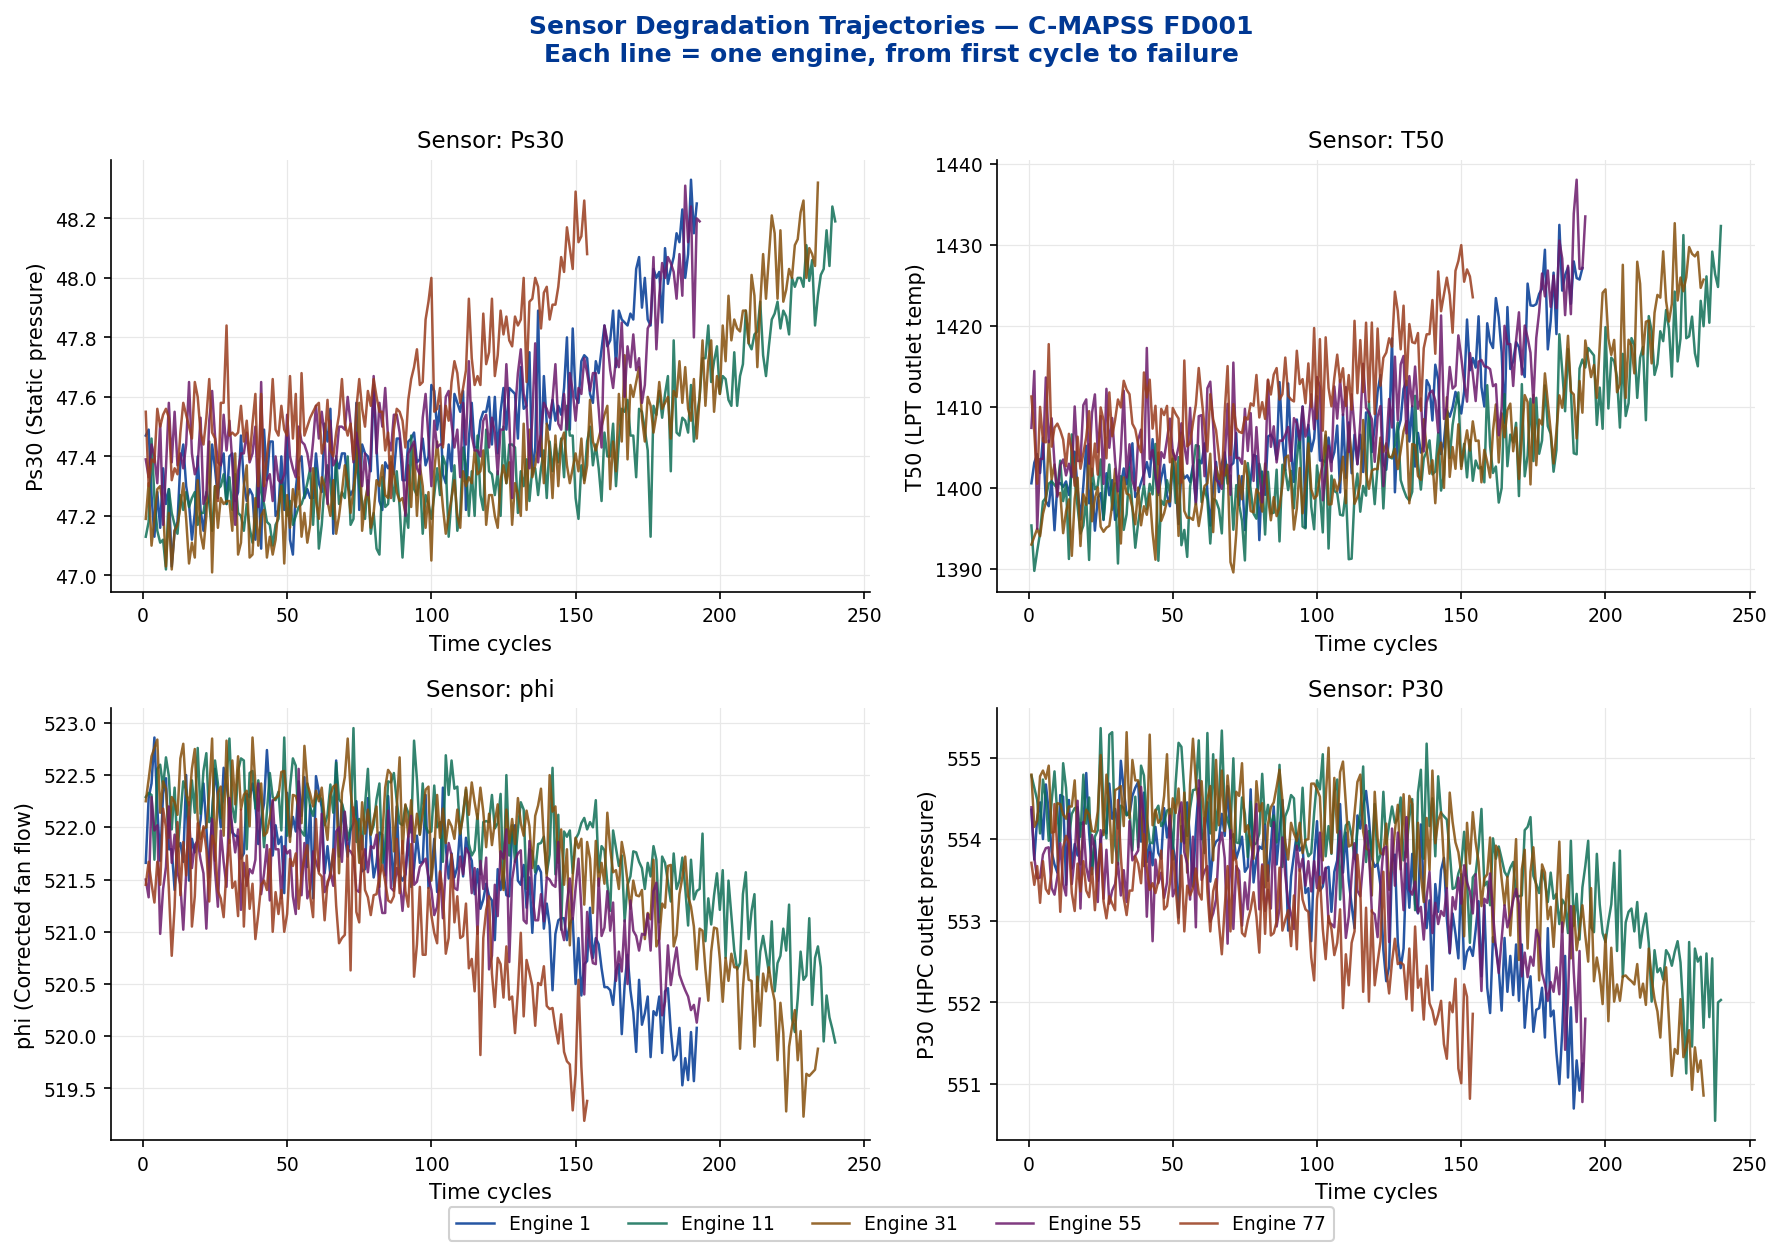
\includegraphics[width=0.95\textwidth]{images/plot_A1_degradation.png}
  \caption{Trajektori degradasi sensor FD001 untuk lima mesin ---
    sensor Ps30, T50, phi, dan P30 menunjukkan \textit{drift}
    yang jelas menjelang akhir umur mesin;
    setiap mesin memiliki panjang hidup berbeda}
  \label{fig:degradation}
\end{figure}

Setiap mesin memiliki umur total berbeda (panjang x-axis berbeda).
Sensor menunjukkan nilai yang relatif stabil di fase sehat, kemudian
mulai menyimpang di fase degradasi. Model harus belajar mengenali
pola penyimpangan ini untuk memprediksi berapa siklus tersisa.

\subsection{Struktur HDF5}

\begin{figure}[H]
  \centering
  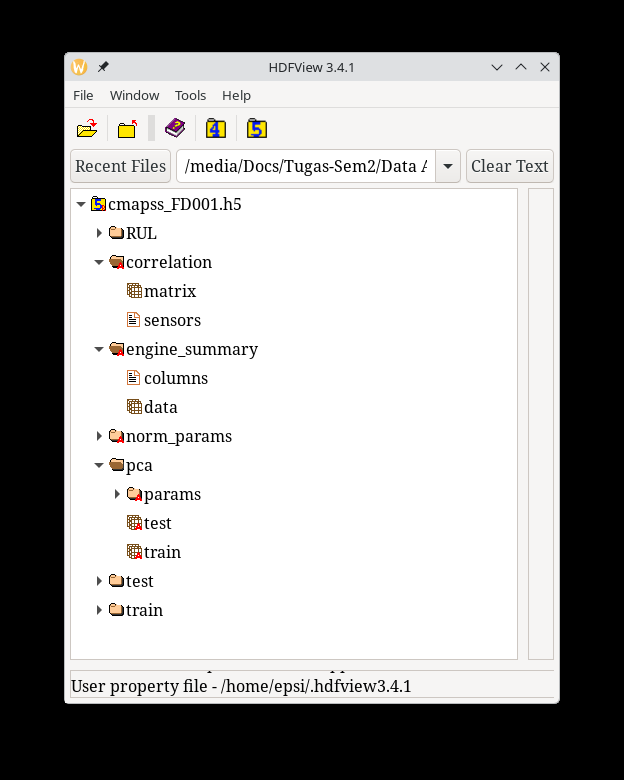
\includegraphics[width=0.40\textwidth]{images/hdf5-05-pca-01-main.png}
  \caption{Struktur HDF5 lengkap \texttt{cmapss\_FD001.h5} di HDFView ---
    dibangun dari raw \texttt{.txt} NASA dalam satu skrip konsolidasi}
  \label{fig:hdf5}
\end{figure}

% ══════════════════════════════════════════════════════════════════════════════
\section{Pembersihan Data}

\subsection{Metode: Korelasi Sensor terhadap Output RUL}

Pembersihan data dilakukan dengan menganalisis hubungan setiap sensor
terhadap output (RUL) menggunakan lima metode statistik:

\begin{enumerate}[noitemsep]
  \item \textbf{Standar Deviasi} --- sensor konstan (std $= 0$) tidak bervariasi
  \item \textbf{Koefisien Variasi (CV)} --- $\text{CV} = \sigma/|\mu|$
  \item \textbf{Korelasi Pearson vs RUL} --- hubungan linear sensor terhadap output
  \item \textbf{Korelasi Spearman vs RUL} --- hubungan monoton terhadap output
  \item \textbf{Mutual Information vs RUL} --- hubungan non-linear terhadap output
\end{enumerate}

\subsection{Hasil Analisis}

\begin{table}[H]
\centering\small
\caption{Statistik 21 sensor FD001 terhadap output RUL ---
  sensor dengan std $= 0$ ($\dagger$) dieliminasi}
\label{tab:sensor_stats}
\begin{tabular}{lrrrrrrl}
\toprule
Sensor & Mean & Std & CV & Pearson & Spearman & MI & Hapus \\
\midrule
T2$^\dagger$         & 518.67 & 0.000 & 0.000 & NaN     & NaN     & 0.000 & \checkmark \\
T24          & 642.68 & 0.500 & 0.001 & $-$0.607 & $-$0.629 & 0.342 & \\
T30          & 1590.5 & 6.131 & 0.004 & $-$0.585 & $-$0.606 & 0.306 & \\
T50          & 1408.9 & 9.001 & 0.006 & $-$0.679 & $-$0.702 & 0.467 & \\
P2$^\dagger$         &  14.62 & 0.000 & 0.000 & NaN     & NaN     & 0.006 & \checkmark \\
P15          &  21.61 & 0.001 & 0.000 & $-$0.128 & $-$0.128 & 0.006 & \checkmark \\
P30          & 553.37 & 0.885 & 0.002 & $+$0.657 & $+$0.679 & 0.425 & \\
Nf           & 2388.1 & 0.071 & 0.000 & $-$0.564 & $-$0.574 & 0.258 & \\
Nc           & 9065.2 & 22.08 & 0.002 & $-$0.390 & $-$0.322 & 0.222 & \\
epr$^\dagger$        &   1.30 & 0.000 & 0.000 & NaN     & NaN     & 0.000 & \checkmark \\
Ps30         &  47.54 & 0.267 & 0.006 & $-$0.696 & $-$0.718 & 0.507 & \\
phi          & 521.41 & 0.738 & 0.001 & $+$0.672 & $+$0.693 & 0.442 & \\
NRf          & 2388.1 & 0.072 & 0.000 & $-$0.563 & $-$0.573 & 0.262 & \\
NRc          & 8143.8 & 19.08 & 0.002 & $-$0.307 & $-$0.202 & 0.225 & \\
BPR          &   8.44 & 0.038 & 0.004 & $-$0.643 & $-$0.666 & 0.390 & \\
farB$^\dagger$       &   0.03 & 0.000 & 0.000 & NaN     & NaN     & 0.000 & \checkmark \\
htBleed      & 393.21 & 1.549 & 0.004 & $-$0.606 & $-$0.629 & 0.328 & \\
Nf\_dmd$^\dagger$    & 2388.0 & 0.000 & 0.000 & NaN     & NaN     & 0.000 & \checkmark \\
PCNfR\_dmd$^\dagger$ & 100.00 & 0.000 & 0.000 & NaN     & NaN     & 0.000 & \checkmark \\
W31          &  38.82 & 0.181 & 0.005 & $+$0.629 & $+$0.653 & 0.367 & \\
W32          &  23.29 & 0.108 & 0.005 & $+$0.636 & $+$0.657 & 0.380 & \\
\bottomrule
\multicolumn{8}{l}{\small $^\dagger$ std $= 0$:
  Pearson/Spearman tidak terdefinisi (NaN); tidak ada korelasi dengan RUL}
\end{tabular}
\end{table}

Enam sensor dieliminasi karena std $= 0$: T2, P2, epr, farB, Nf\_dmd,
PCNfR\_dmd. Sensor P15 juga dieliminasi karena Pearson $= -0{,}13$
(hampir tidak ada korelasi linear dengan RUL).
Tersisa \textbf{15 sensor} aktif.

% ══════════════════════════════════════════════════════════════════════════════
\section{Normalisasi}

\subsection{Metode Z-Score Berbasis Siklus Sehat}

\begin{equation}
  z = \frac{x - \mu_{\text{healthy}}}{\sigma_{\text{healthy}}}
\end{equation}

Parameter $\mu$ dan $\sigma$ dihitung hanya dari siklus dengan
RUL\_raw $\geq 125$ (\textit{healthy cycles}).

\begin{figure}[H]
  \centering
  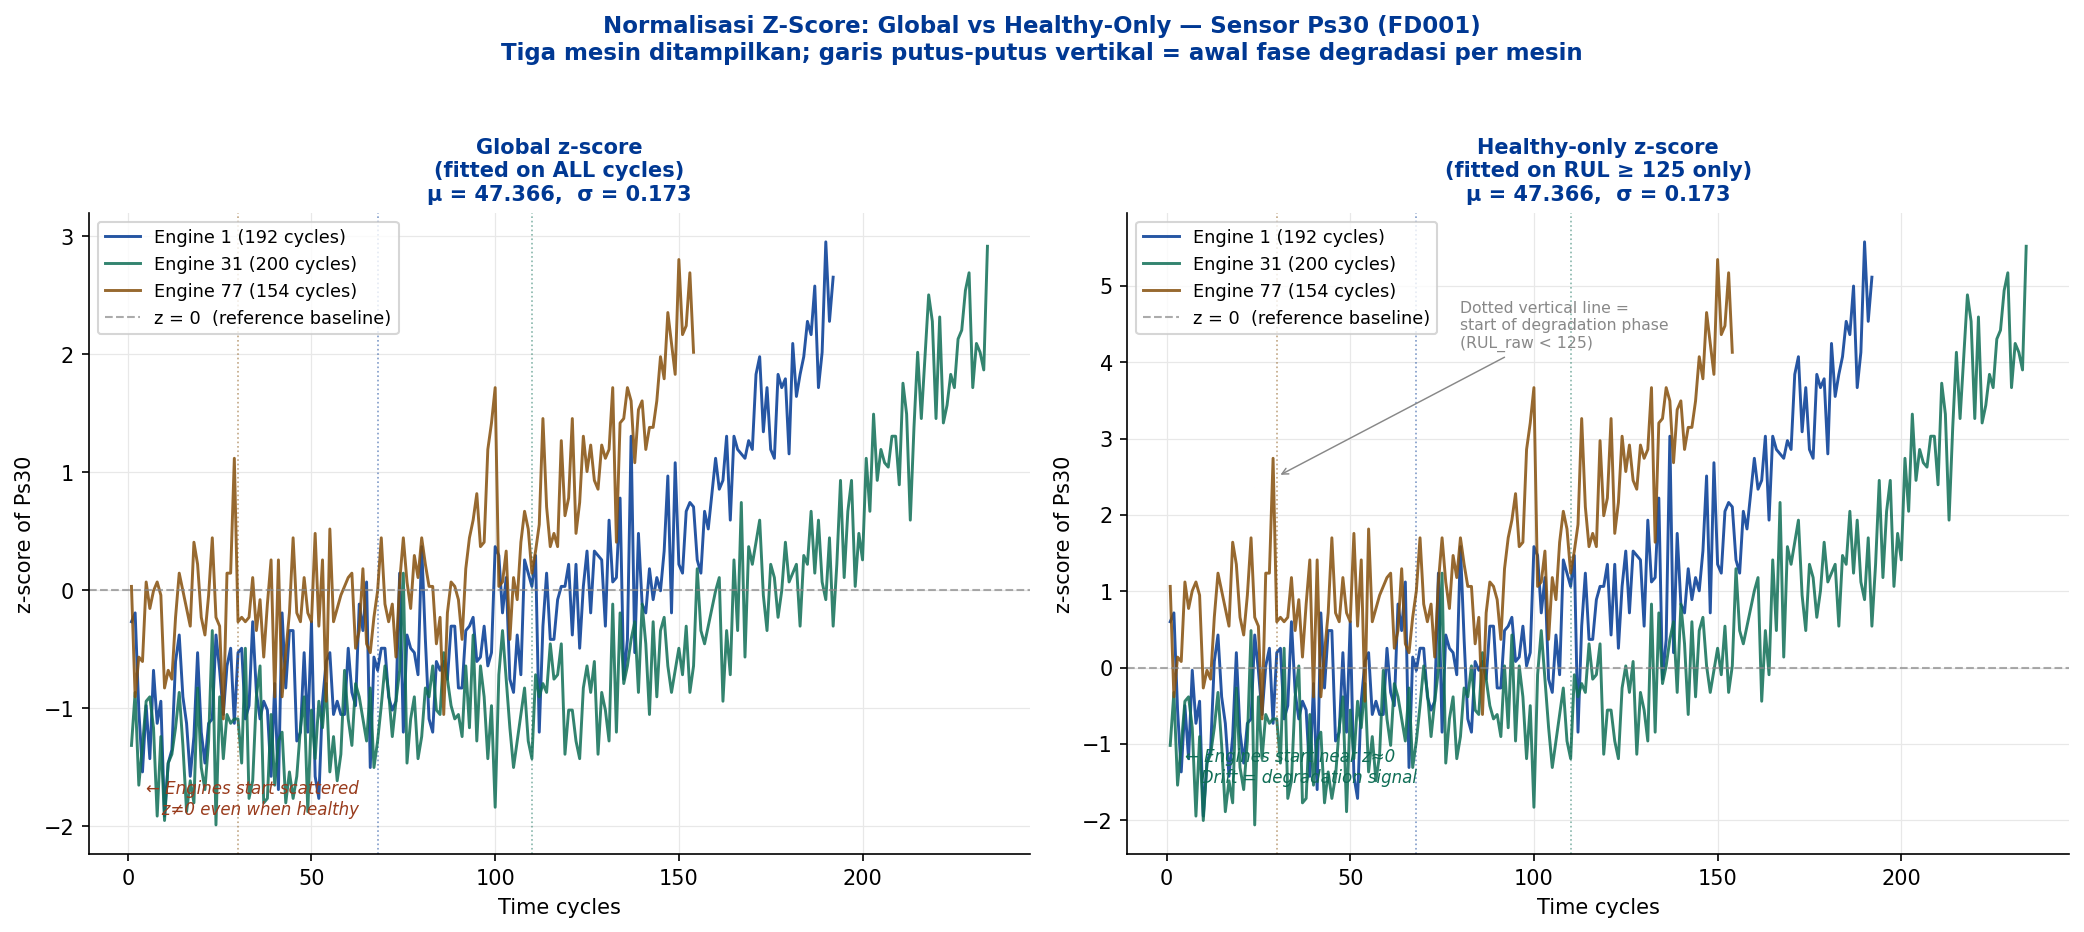
\includegraphics[width=0.96\textwidth]{images/plot_D13_norm_comparison.png}
  \caption{Perbandingan normalisasi global vs \textit{healthy-only}
    untuk sensor Ps30 pada tiga mesin FD001
    (Engine 1 biru 192 siklus, Engine 31 hijau $\approx$200 siklus,
    Engine 77 coklat 154 siklus) ---
    garis putus-putus vertikal = awal fase degradasi per mesin
    (saat RUL\_raw $< 125$)}
  \label{fig:norm_comparison}
\end{figure}

Gambar \ref{fig:norm_comparison} membandingkan dua metode normalisasi
pada sensor Ps30 untuk tiga mesin. \textbf{Global z-score (kiri)}:
ketiga mesin mulai tersebar di nilai z berbeda --- referensi nol
tidak konsisten karena $\mu$ dipengaruhi siklus terdegradasi.
\textbf{Healthy-only z-score (kanan)}: ketiga mesin mulai di
$z \approx 0$ lalu secara konsisten \textit{drift} ke atas seiring
degradasi --- penyimpangan dari nol inilah sinyal yang dipelajari model.

Data \textit{test} dinormalisasi menggunakan parameter dari
\textit{train} untuk menghindari \textit{data leakage}.

% ══════════════════════════════════════════════════════════════════════════════
\section{Seleksi Fitur}

\subsection{Korelasi Pearson Antar Sensor}

\begin{figure}[H]
  \centering
  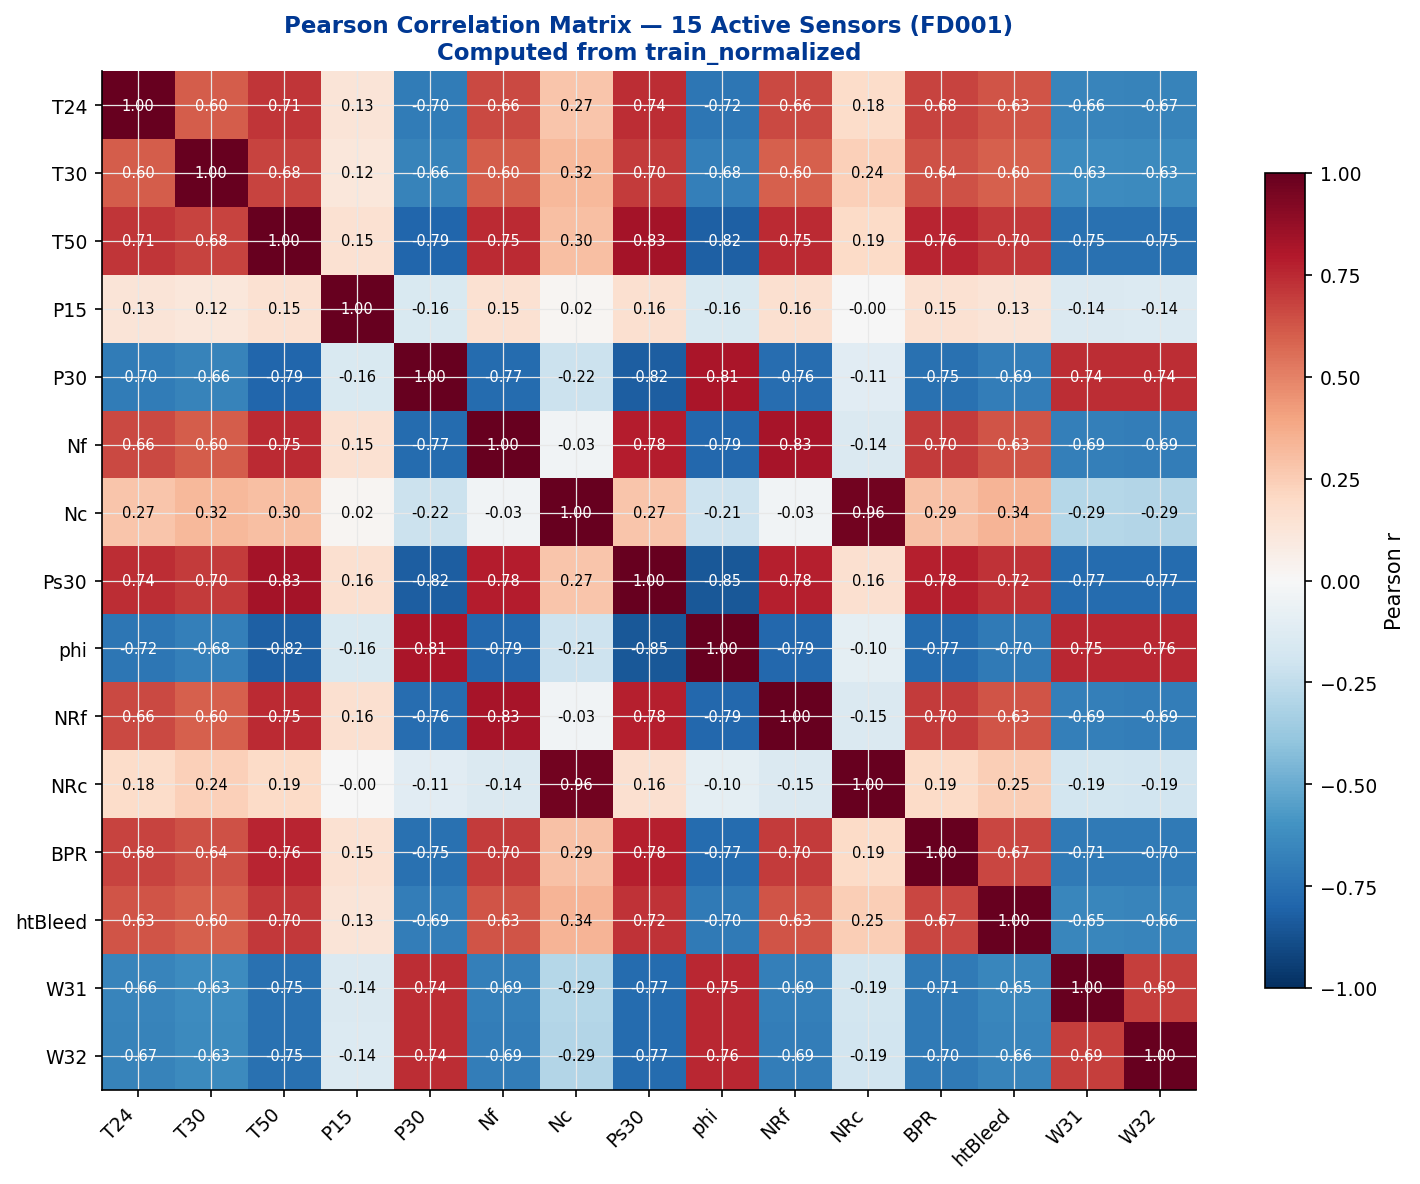
\includegraphics[width=0.82\textwidth]{images/plot_A2_correlation.png}
  \caption{Matriks korelasi Pearson antar 15 sensor aktif FD001 ---
    blok merah gelap pada Nc--NRc ($r = 0{,}96$) dan Nf--NRf
    ($r = 0{,}83$) menunjukkan redundansi tinggi yang memotivasi PCA}
  \label{fig:corr}
\end{figure}

\subsection{Principal Component Analysis (PCA)}

\begin{figure}[H]
  \centering
  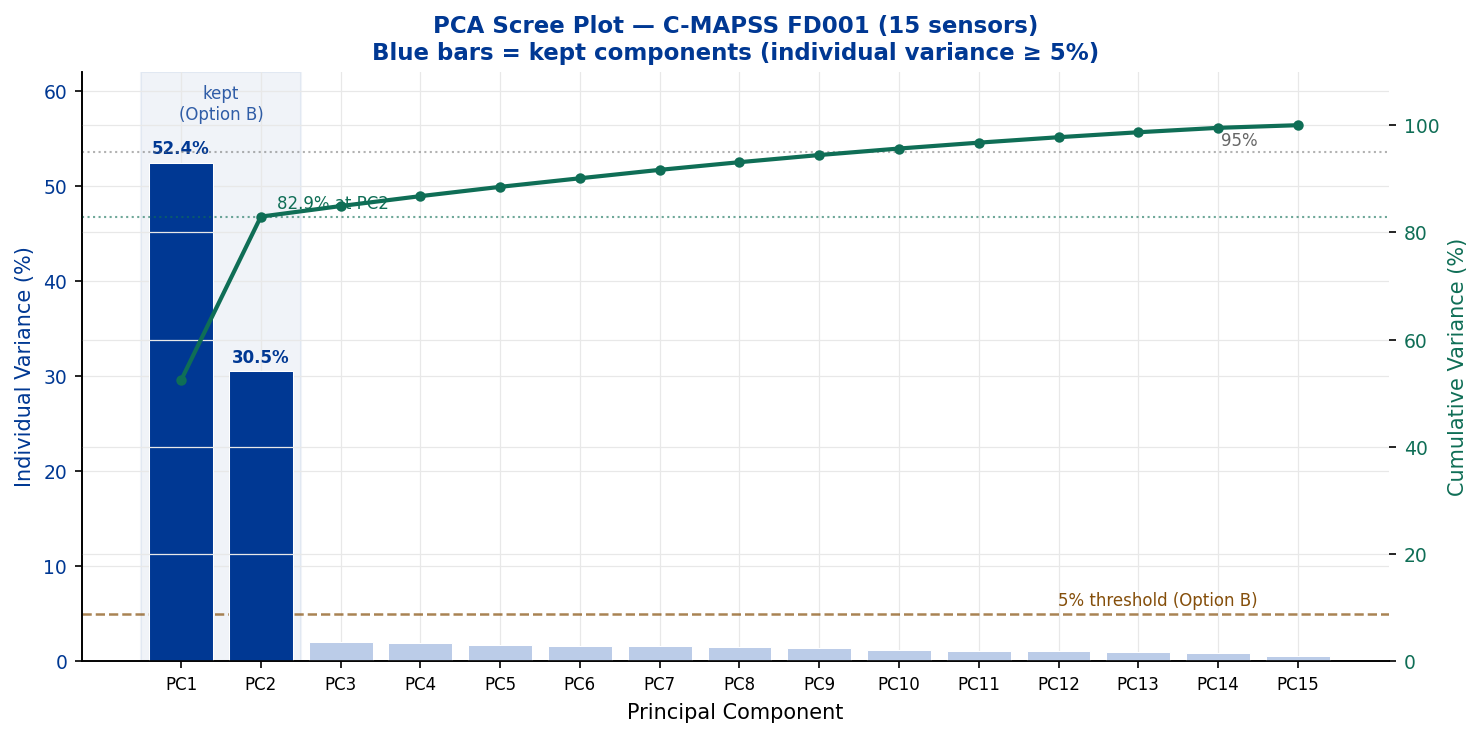
\includegraphics[width=0.88\textwidth]{images/plot_A3_scree.png}
  \caption{\textit{Scree plot} PCA FD001 --- \textit{cliff} tajam
    setelah PC2 (52,4\% + 30,5\% = 82,9\%) menunjukkan
    PC3 dan seterusnya hanya mengandung \textit{noise};
    2 komponen dipertahankan (varians individual $\geq 5\%$)}
  \label{fig:scree}
\end{figure}

\begin{table}[H]
\centering\small
\caption{Varians PCA FD001 (15 sensor $\to$ 2 komponen dipertahankan)}
\label{tab:pca_var}
\begin{tabular}{lrrrrrrrr}
\toprule
& PC1 & PC2 & PC3 & PC4 & PC5 & PC6 & PC7 & PC8 \\
\midrule
Individual & 52,4\% & 30,5\% & 2,0\% & 1,8\% & 1,7\% & 1,6\% & 1,6\% & 1,4\% \\
Kumulatif  & 52,4\% & 82,9\% & 84,9\% & 86,7\% & 88,4\% & 90,1\% & 91,7\% & 93,0\% \\
\bottomrule
\end{tabular}
\end{table}

\begin{figure}[H]
  \centering
  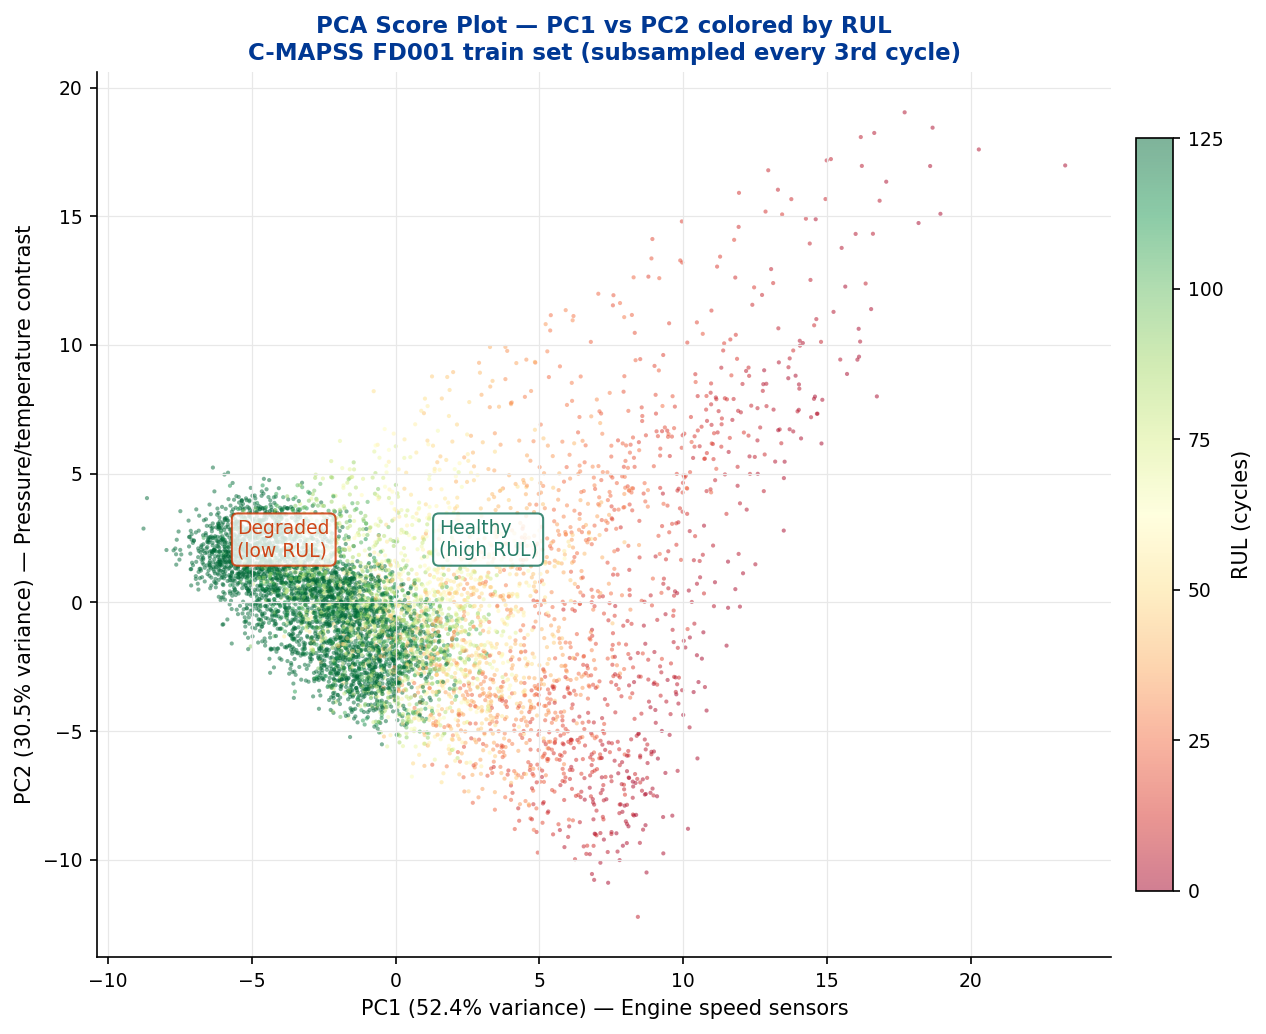
\includegraphics[width=0.82\textwidth]{images/plot_A4_pca_scatter.png}
  \caption{\textit{Scatter plot} PC1 vs PC2 diwarnai berdasarkan RUL
    (hijau = sehat, merah = mendekati gagal) ---
    setiap titik adalah satu siklus mesin;
    warna merepresentasikan RUL sebagai dimensi ketiga;
    titik hijau (sehat) cenderung ke kanan, merah (degraded) ke kiri}
  \label{fig:pca_scatter}
\end{figure}

PC1 (52,4\%) didominasi sensor kecepatan poros Nf, NRf, Nc, NRc ---
merepresentasikan \textit{overall engine speed state}. PC2 (30,5\%)
merepresentasikan kontras tekanan-kecepatan.

\subsection{Pipeline Spreadsheet}

\begin{figure}[H]
  \centering
  \begin{subfigure}[b]{0.48\textwidth}
    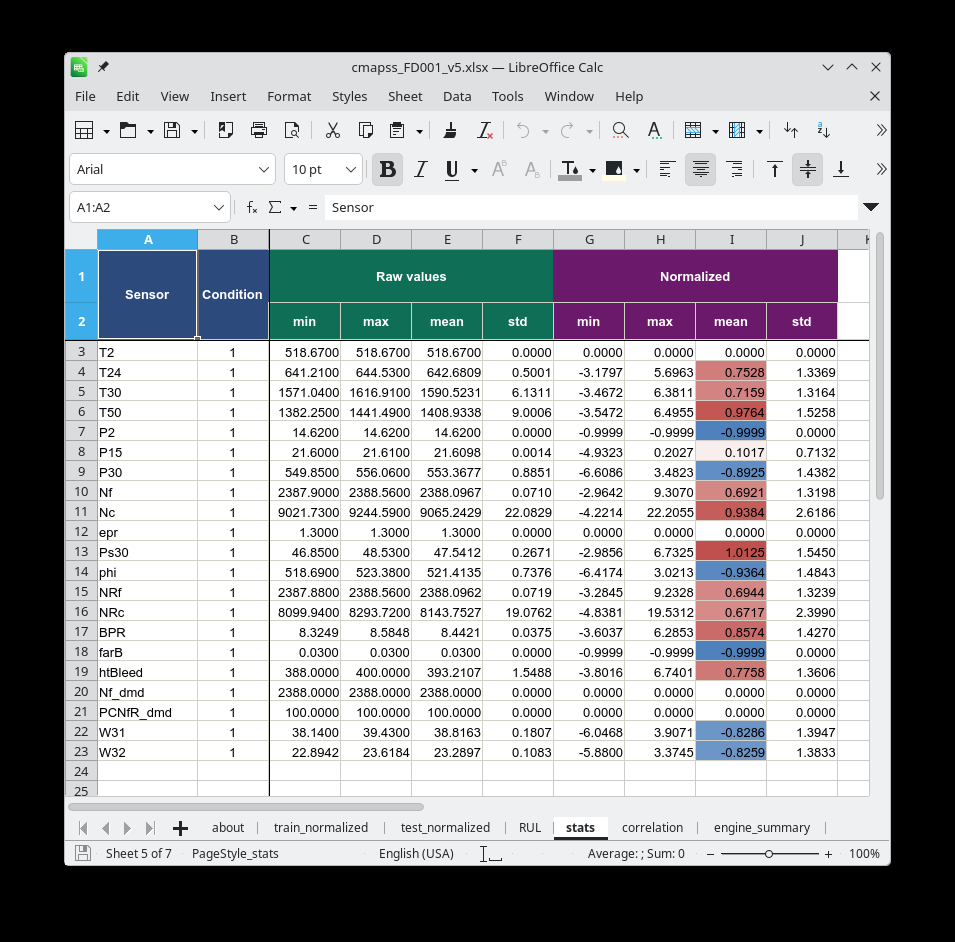
\includegraphics[width=\textwidth]{images/workbook-05-correlation-04-statistics.png}
    \caption{Sheet \texttt{stats} (v5)}
  \end{subfigure}
  \hfill
  \begin{subfigure}[b]{0.48\textwidth}
    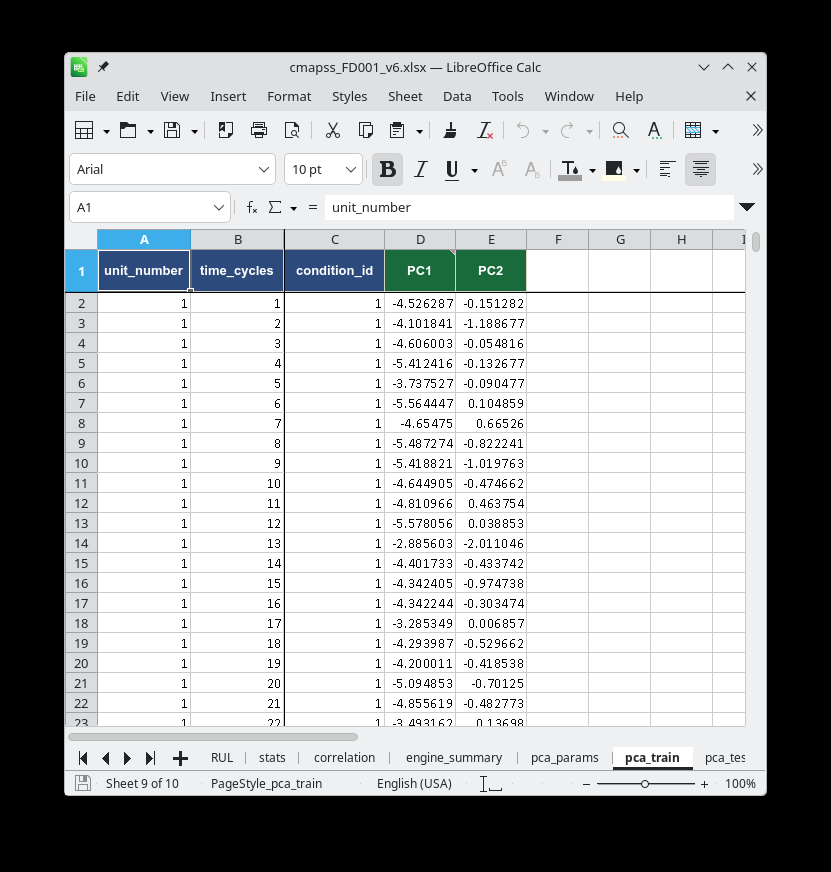
\includegraphics[width=\textwidth]{images/workbook-06-pca-12-pca-train.png}
    \caption{Sheet \texttt{pca\_train} (v6)}
  \end{subfigure}
  \caption{Spreadsheet v5 dan v6 --- dari statistik sensor
    hingga skor PC per siklus}
  \label{fig:spreadsheet}
\end{figure}

% ══════════════════════════════════════════════════════════════════════════════
\section{Model \textit{Artificial Neural Network}}

\subsection{Arsitektur dan Konfigurasi}

\begin{figure}[H]
  \centering
  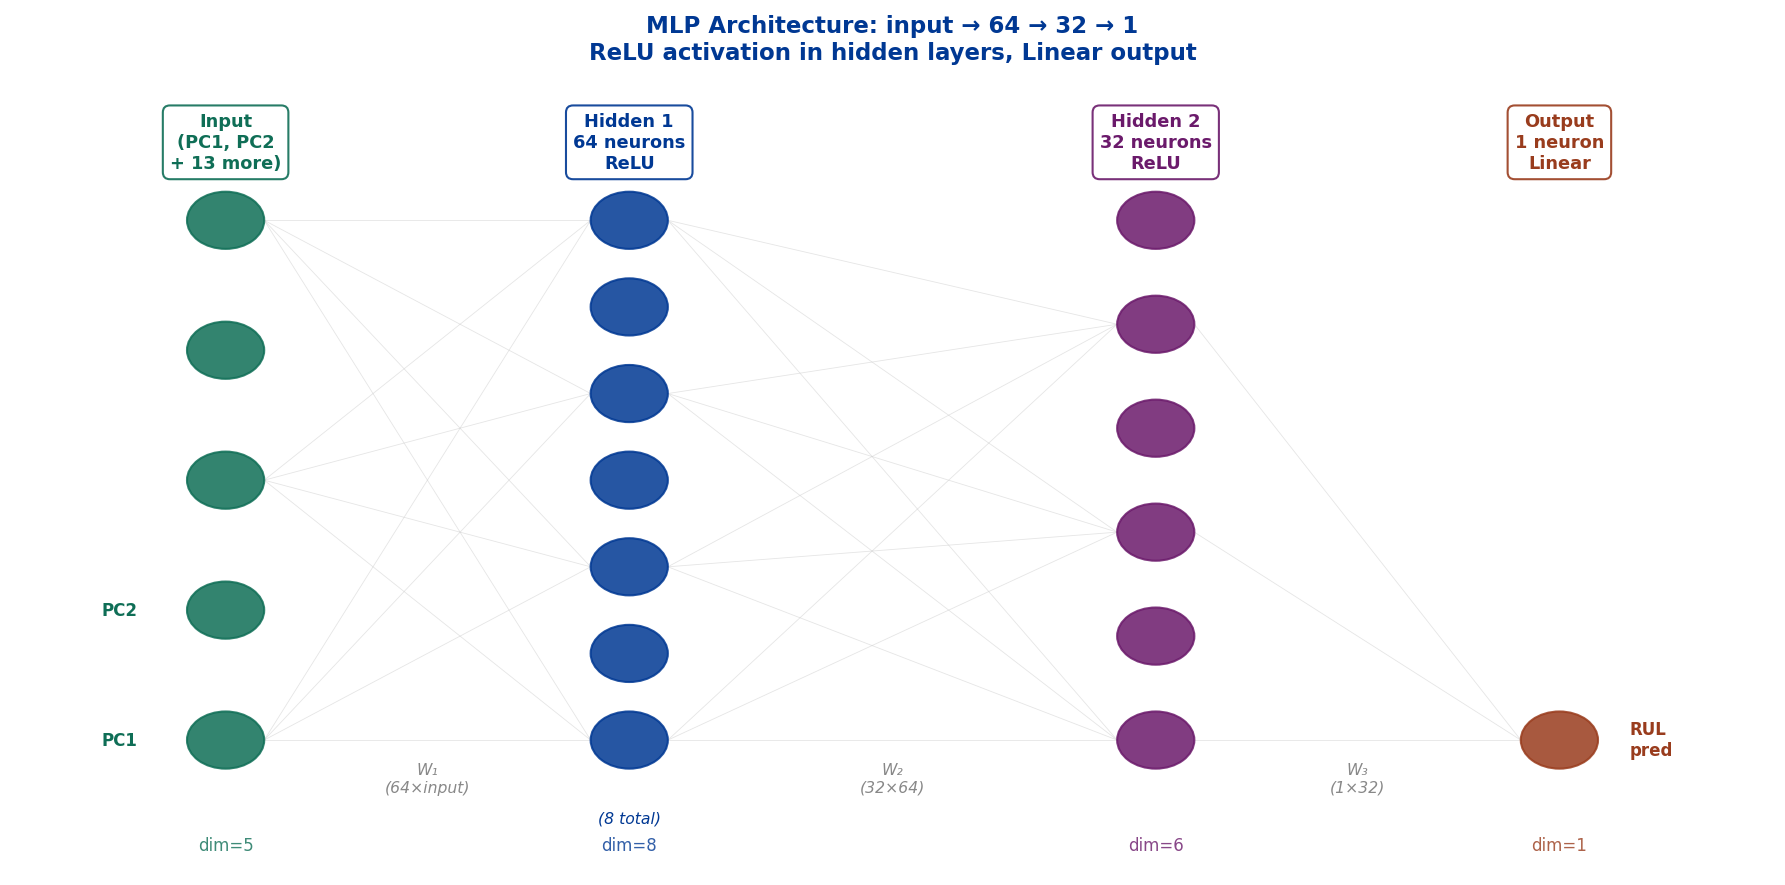
\includegraphics[width=0.88\textwidth]{images/plot_D14_mlp_arch.png}
  \caption{Arsitektur MLP: input $\to$ 64 $\to$ 32 $\to$ 1 ---
    ReLU pada lapisan tersembunyi, output linear}
  \label{fig:mlp_arch}
\end{figure}

\begin{table}[H]
\centering\small
\caption{Konfigurasi pelatihan ANN}
\label{tab:ann_config}
\begin{tabular}{ll}
\toprule
Parameter & Nilai \\
\midrule
Arsitektur    & input $\to$ 64 $\to$ 32 $\to$ 1 \\
Aktivasi      & ReLU (tersembunyi), Linear (output) \\
\textit{Loss} & MSE \\
Optimizer     & Adam, lr $= 10^{-3}$ \\
Epoch         & 500  \quad Batch size: 512 \\
Target        & RUL\_capped (cap $= 125$ siklus) \\
\bottomrule
\end{tabular}
\end{table}

\subsection{Target: RUL Capped}

\begin{figure}[H]
  \centering
  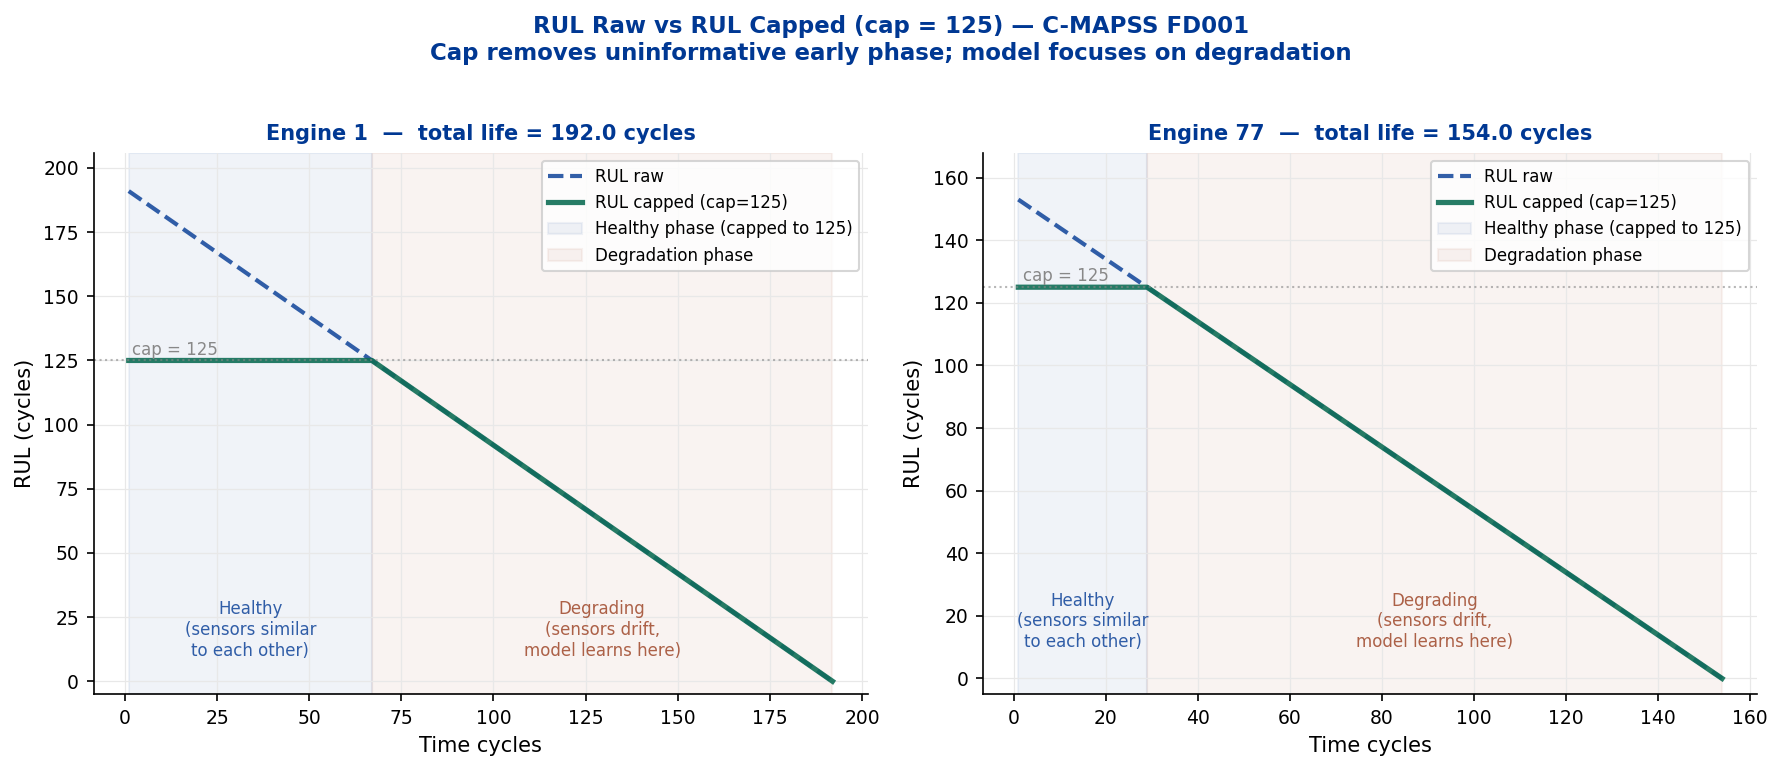
\includegraphics[width=0.88\textwidth]{images/plot_D12_rul_cap.png}
  \caption{RUL raw vs RUL capped untuk Engine 1 (192 siklus) dan
    Engine 77 (154 siklus) ---
    dua mesin ditampilkan untuk membuktikan cap bekerja konsisten
    terlepas dari panjang hidup mesin;
    fase sehat (biru) diratakan ke 125 pada kedua mesin}
  \label{fig:rul_cap}
\end{figure}

\subsection{NASA Score}

\begin{figure}[H]
  \centering
  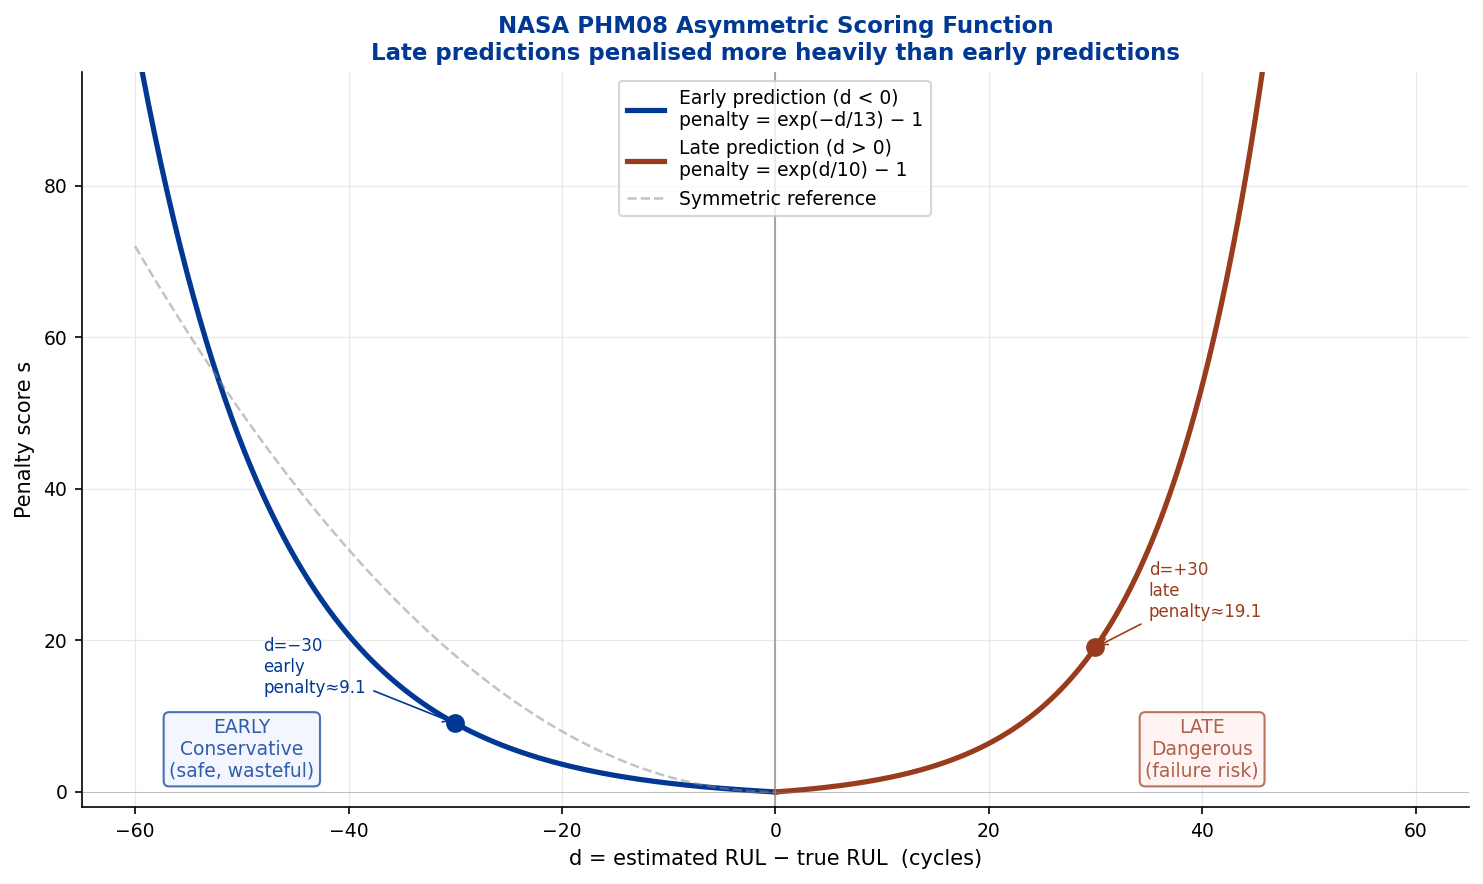
\includegraphics[width=0.72\textwidth]{images/plot_D11_nasa_score.png}
  \caption{Kurva penalti NASA Score --- prediksi \textit{late}
    ($d > 0$, merah) dihukum lebih berat karena membahayakan
    keselamatan; prediksi \textit{early} ($d < 0$, biru) lebih ringan}
  \label{fig:nasa_score}
\end{figure}

\subsection{Dua Model yang Dibandingkan}

\begin{itemize}[noitemsep]
  \item \textbf{Model PCA}: input = PC1, PC2 (2 fitur)
  \item \textbf{Model NORM}: input = 15 sensor ternormalisasi
\end{itemize}

\subsection{Hasil Training}

\begin{figure}[H]
  \centering
  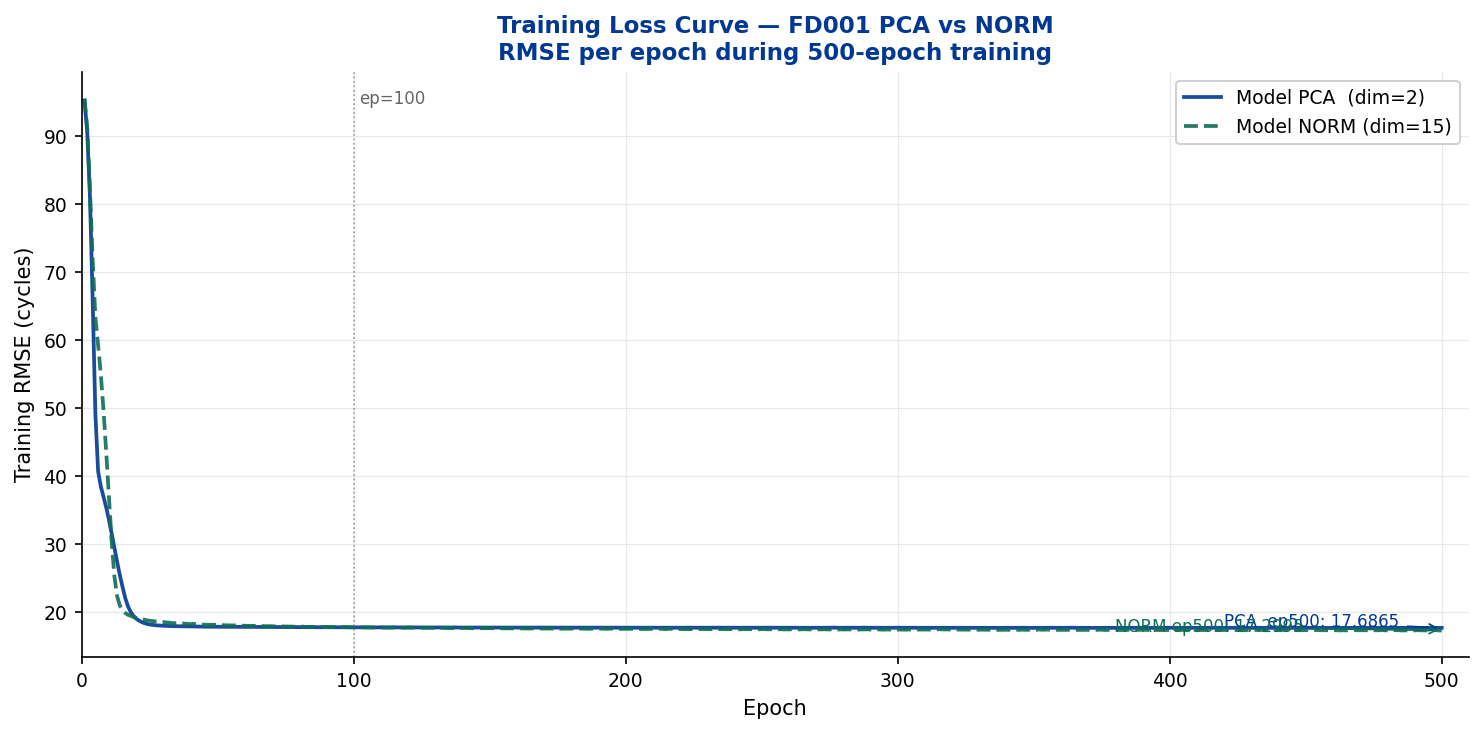
\includegraphics[width=0.88\textwidth]{images/plot_B5_loss_curve.png}
  \caption{Kurva \textit{loss} (training RMSE per epoch) ---
    Model PCA (biru) konvergen lebih cepat karena input lebih kecil
    (2 vs 15 fitur); keduanya konvergen baik setelah 300 epoch}
  \label{fig:loss_curve}
\end{figure}

\subsection{Hasil}

\begin{table}[H]
\centering\small
\caption{Perbandingan dua model FD001 (500 epoch, batch 512)}
\label{tab:results}
\begin{tabular}{lcrrrr}
\toprule
Model & Input & Dim & RMSE & MAE & NASA Score \\
\midrule
\textbf{FD001\_PCA}  & PC1, PC2  & 2  &
  \textbf{17,80} & \textbf{12,55} & \textbf{815} \\
FD001\_NORM & 15 sensor & 15 &
  18,21 & 13,52 & 929 \\
\bottomrule
\end{tabular}
\end{table}

\begin{figure}[H]
  \centering
  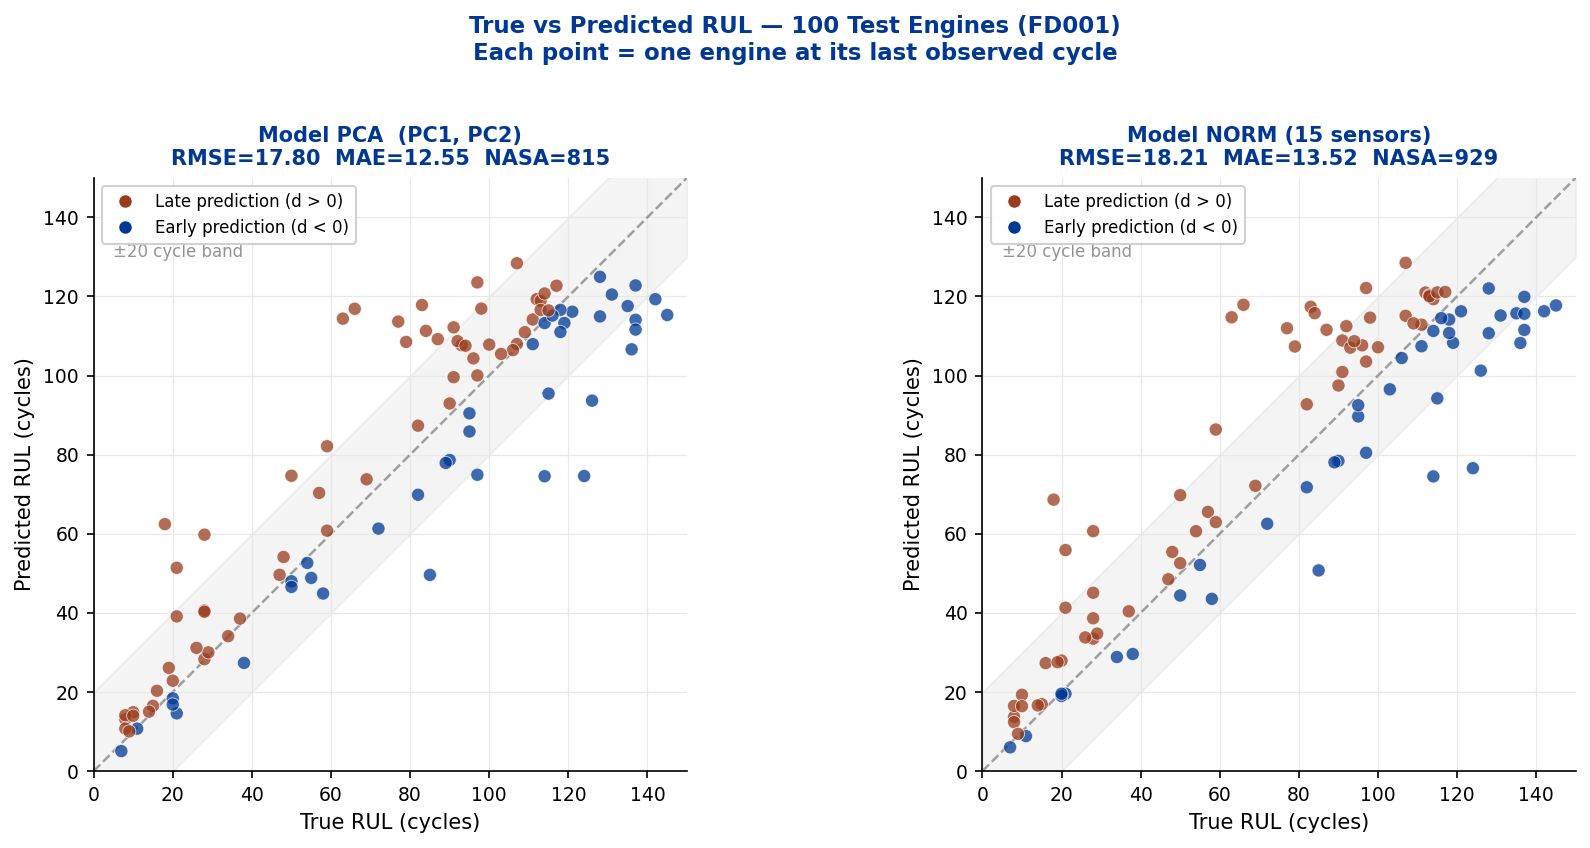
\includegraphics[width=0.90\textwidth]{images/plot_B6_true_vs_pred.png}
  \caption{True vs Predicted RUL untuk 100 mesin \textit{test} ---
    garis diagonal = prediksi sempurna;
    titik merah = prediksi \textit{late} (di atas diagonal),
    titik biru = prediksi \textit{early} (di bawah diagonal);
    pola linear karena target RUL sendiri adalah \textit{countdown} linear}
  \label{fig:true_pred}
\end{figure}

\begin{figure}[H]
  \centering
  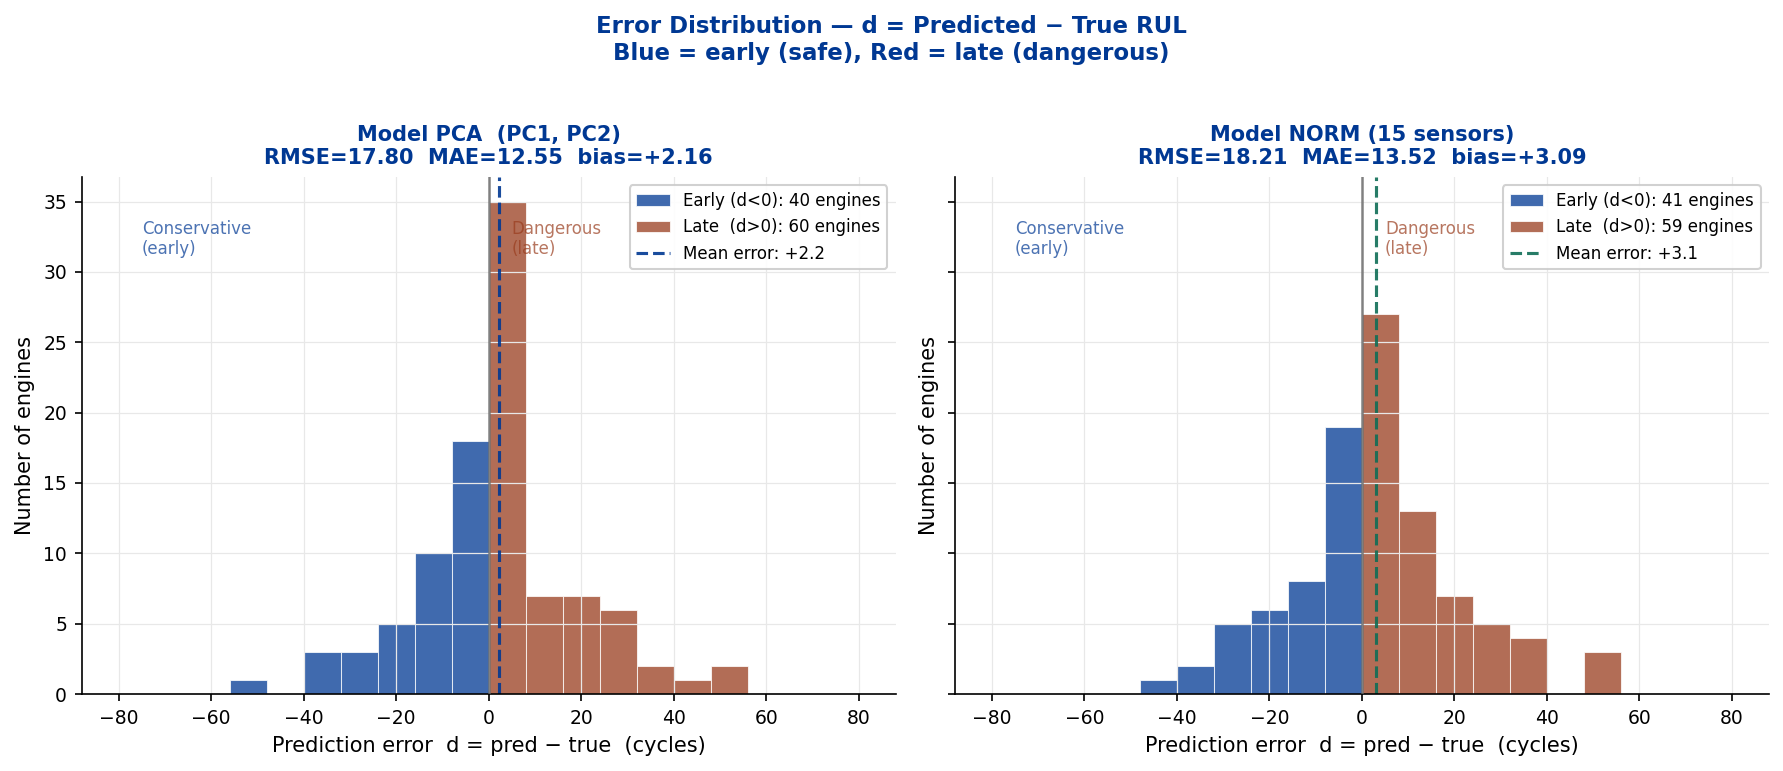
\includegraphics[width=0.88\textwidth]{images/plot_B7_error_dist.png}
  \caption{Distribusi error prediksi ($d = \text{pred} - \text{true}$) ---
    distribusi \textit{right-skewed} menunjukkan bias prediksi \textit{late};
    Model PCA memiliki distribusi lebih sempit dan bias lebih kecil}
  \label{fig:error_dist}
\end{figure}

Model PCA mengungguli NORM pada ketiga metrik. Kompresi PCA
(82,9\% varians dalam 2 komponen) efektif membuang \textit{noise}
pada FD001 yang sederhana (1 kondisi, 1 mode kerusakan).

% ══════════════════════════════════════════════════════════════════════════════
\section{Analisis Garson}

\subsection{Algoritma Garson}

Algoritma Garson \cite{garson1991} menghitung kepentingan relatif
fitur input berdasarkan bobot jaringan terlatih:

\begin{align}
  q_1[i,j] &= \frac{|W_1[j,i]|}{\sum_k |W_1[j,k]|} &
  q_2[j,m] &= \frac{|W_2[m,j]|}{\sum_k |W_2[m,k]|} \\[4pt]
  r[i,m]   &= \sum_j q_1[i,j] \cdot q_2[j,m] &
  s[i]     &= \sum_m r[i,m] \cdot |W_3[m]| \\[4pt]
  \text{importance}[i] &= \frac{s[i]}{\sum_k s[k]}
\end{align}

\subsection{Hasil Model PCA}

\begin{figure}[H]
  \centering
  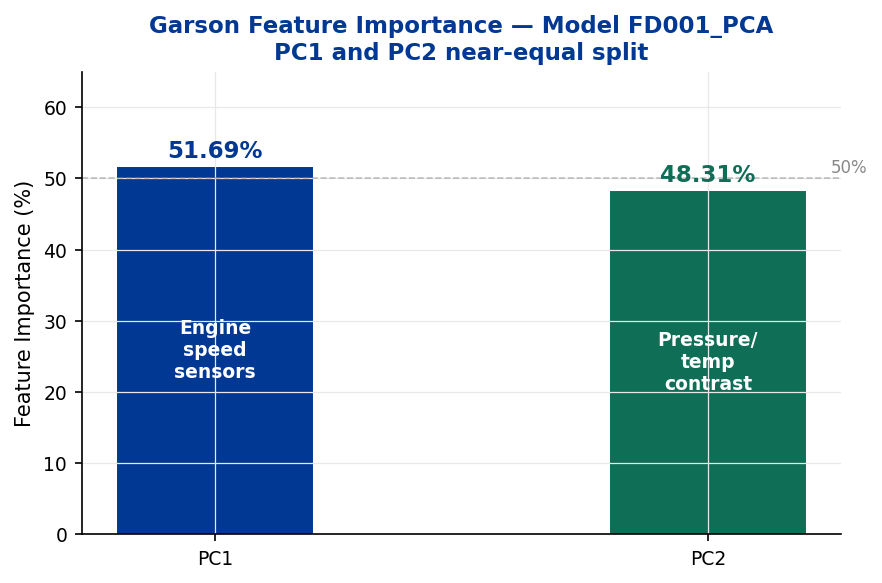
\includegraphics[width=0.52\textwidth]{images/plot_C10_garson_pca.png}
  \caption{Kepentingan Garson Model FD001\_PCA ---
    PC1 dan PC2 hampir seimbang (51,69\% vs 48,31\%);
    kedua komponen sama-sama penting}
  \label{fig:garson_pca}
\end{figure}

\subsection{Hasil Model NORM}

\begin{figure}[H]
  \centering
  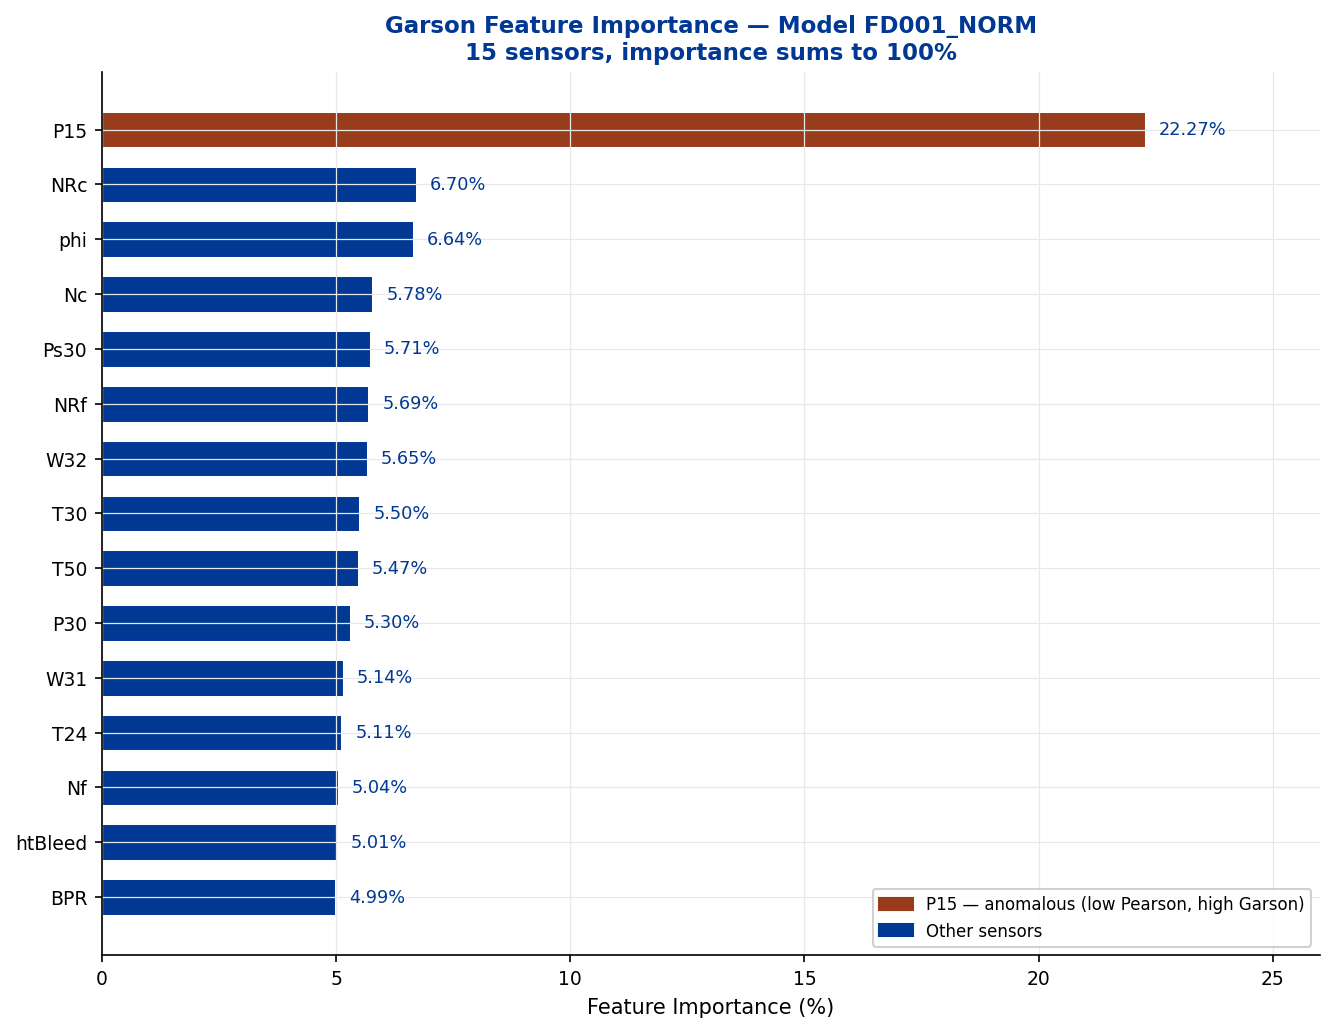
\includegraphics[width=0.88\textwidth]{images/plot_C8_garson_norm.png}
  \caption{Kepentingan Garson Model FD001\_NORM ---
    P15 mendominasi dengan 22,27\% meskipun korelasi Pearson
    hanya $-0{,}13$; ANN menemukan sinyal non-linear}
  \label{fig:garson_norm}
\end{figure}

\subsection{Perbandingan Tiga Metode}

\begin{figure}[H]
  \centering
  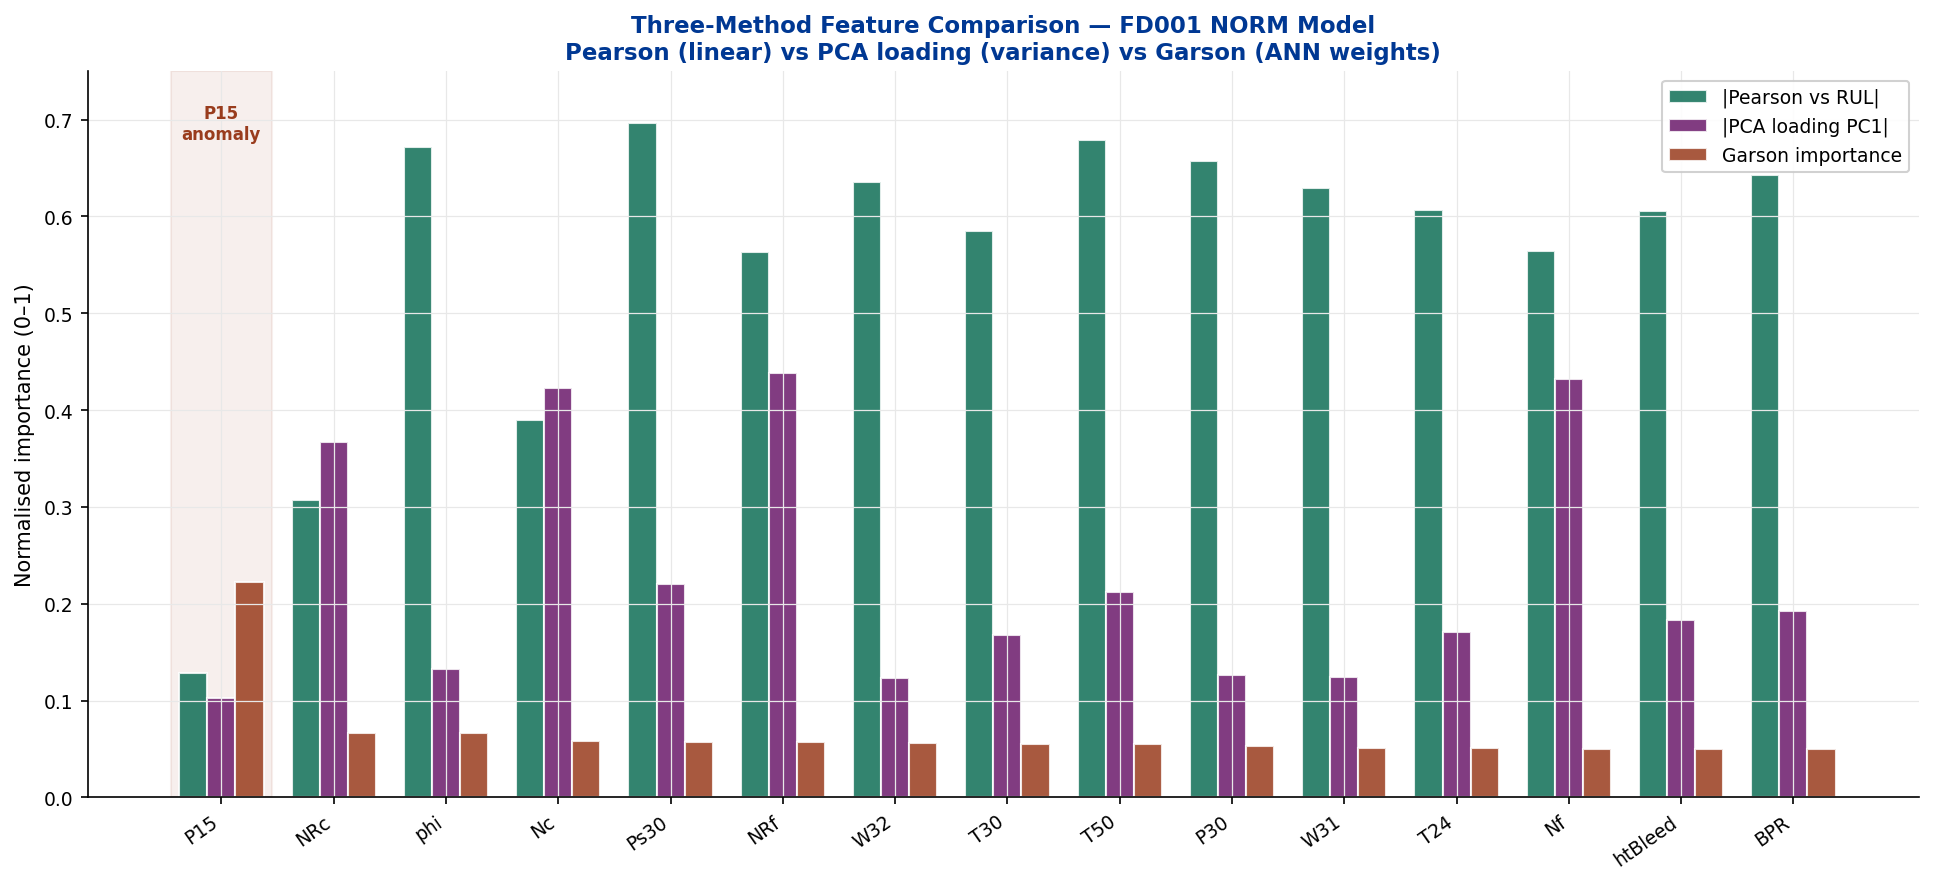
\includegraphics[width=0.95\textwidth]{images/plot_C9_three_method.png}
  \caption{Perbandingan tiga metode seleksi fitur ---
    teal = $|$Pearson vs RUL$|$, ungu = $|$PCA loading$|$,
    merah = Garson; area diarsir = anomali P15 yang hanya
    terdeteksi oleh Garson}
  \label{fig:three_method}
\end{figure}

\begin{table}[H]
\centering\small
\caption{Perbandingan tiga metode untuk sensor pilihan (FD001)}
\label{tab:three_method}
\begin{tabular}{lcccp{5cm}}
\toprule
Sensor & Pearson & PCA Loading & Garson & Interpretasi \\
\midrule
Ps30   & $-0{,}70$ & tinggi & sedang & Konsisten --- penting secara linear \\
T50    & $-0{,}68$ & tinggi & sedang & Konsisten --- penting secara linear \\
P30    & $+0{,}66$ & tinggi & sedang & Konsisten --- penting secara linear \\
\textbf{P15}
       & $-0{,}13$ & rendah & \textbf{22,27\%}
  & \textbf{Anomali} --- sinyal non-linear terdeteksi ANN \\
\bottomrule
\end{tabular}
\end{table}

Temuan utama: sensor P15 memiliki Pearson rendah dan PCA loading rendah,
namun Garson menetapkannya sebagai fitur terpenting (22,27\%). ANN
mengeksploitasi hubungan non-linear yang tidak terdeteksi oleh
dua metode statistik linear.

% ══════════════════════════════════════════════════════════════════════════════
\section{Kesimpulan}

\begin{enumerate}[noitemsep]
  \item \textbf{Enam sensor dieliminasi} karena std $= 0$ ---
    tidak ada variasi maupun korelasi dengan output RUL.

  \item \textbf{PCA menghasilkan 2 komponen} yang menjelaskan 82,9\%
    varians: PC1 = kecepatan mesin, PC2 = kontras tekanan-kecepatan.

  \item \textbf{Model PCA mengungguli NORM} pada FD001:
    RMSE 17,80 vs 18,21, NASA Score 815 vs 929.

  \item \textbf{Garson mengungkap sinyal non-linear}:
    sensor P15 dengan Pearson $-0{,}13$ terbukti paling penting
    menurut ANN (22,27\%).
\end{enumerate}

% ── References ────────────────────────────────────────────────────────────────
\begin{thebibliography}{9}
\bibitem{saxena2008}
  A. Saxena, K. Goebel, D. Simon, N. Eklund,
  ``Damage Propagation Modeling for Aircraft Engine Run-to-Failure Simulation,''
  \textit{Proc.\ 1st Int.\ Conf.\ Prognostics and Health Management (PHM08)},
  Denver, CO, 2008.

\bibitem{garson1991}
  G.D. Garson,
  ``Interpreting Neural Network Connection Weights,''
  \textit{AI Expert}, vol.~6, no.~4, pp.~46--51, 1991.
\end{thebibliography}

\end{document}
